% Licensed to the Apache Software Foundation (ASF) under one or more
% contributor license agreements. See the NOTICE file distributed with
% this work for additional information regarding copyright ownership.
% The ASF licenses this file to You under the Apache License, Version 2.0
% (the ``License''); you may not use this file except in compliance with
% the License. You may obtain a copy of the License at
%
% http://www.apache.org/licenses/LICENSE-2.0
%
% Unless required by applicable law or agreed to in writing, software
% distributed under the License is distributed on an ``AS IS'' BASIS,
% WITHOUT WARRANTIES OR CONDITIONS OF ANY KIND, either express or implied.
% See the License for the specific language governing permissions and
% limitations under the License.

\subsubsection{Livelink Job Options}

In the Livelink-specific tabs, you will have the following additional
settings:

\bigimage{edit-job-tab3}

\ifLivelinkGuide
% Licensed to the Apache Software Foundation (ASF) under one or more
% contributor license agreements. See the NOTICE file distributed with
% this work for additional information regarding copyright ownership.
% The ASF licenses this file to You under the Apache License, Version 2.0
% (the ``License''); you may not use this file except in compliance with
% the License. You may obtain a copy of the License at
%
% http://www.apache.org/licenses/LICENSE-2.0
%
% Unless required by applicable law or agreed to in writing, software
% distributed under the License is distributed on an ``AS IS'' BASIS,
% WITHOUT WARRANTIES OR CONDITIONS OF ANY KIND, either express or implied.
% See the License for the specific language governing permissions and
% limitations under the License.

\begin{itemize}
\label{scheduling}

\item \textbf{Schedule type:} Whether you want to scan every document
once or dynamically recrawl content in your repository. 

When scanning every document once, the crawler marks all documents that
have been previously crawled in this job as potentially to be deleted,
adds all seed documents to its queue and marks them as pending, processes
pending documents, marking them completed as they are ingested, and then
deleted all of the documents that were not recrawled. A document might
not be recrawled because it no longer exists, or the job specification
might have been changed to no longer include the document.

When dynamically recrawling documents, the crawler does not start by
marking all documents as potentially deletable; instead, it begins with
all of the seed documents, and continues adding to its list, periodically
re-adding the initial seed documents. If a document is removed from the
source, it will expire in the expiration interval (see below).

\item \textbf{Expiration Interval (if continuous):} The length of the
interval (in minutes) that the appliance will retain a document
crawled by this job after the document no longer appears in the
repository. After this interval, the missing document will be removed
from the appliance's index and archive. Leave the expiration interval
blank to keep missing documents indexed in GTS.

\item \textbf{Recrawl interval:} If you are dynamically recrawling
documents, how long, in minutes, the crawler should wait before
crawling documents a second time.

\item \textbf{Reseed interval:} If you are dynamically recrawling
documents, how long, in minutes, the crawler should wait before
looking for new documents to crawl. \ifMeridioGuide This connector
identifies all documents for ingestion through seeding; if the reseed
interval is infinite, the job will not ingest documents placed in the
repository during run time. (The job automatically reseeds whenever it
is started.) The default interval of 60 minutes is an appropriate
reseed rate. \fi \ifFilenetGuide This connector identifies documents
for ingestion during seeding. If you change the document inclusion
criteria, reseeding is required to identify new documents. Similarly,
documents placed in the repository while the job is running will not
be identified until the crawl is reseeded.  (The job automatically
reseeds whenever it is started.) The default interval of 60 minutes is
an appropriate reseed rate. \fi

\item \textbf{Scheduled time:} Allows you to define a time you wish
the job to run using a series of selection boxes. The first box refers
to the day of the week you wish the job to run, with an option to have
the job run any day of the week. The second box allows you to select
the start hour, with an option to start the job at any hour. The third
box allows you to specify which minute after the hour that you wish
the job to start. The fourth box allows you to specify what months of
the year you wish the job to run, with an option for the job to run
any month. The last box allows you to specify the day of the month you
wish the job to start, including any day of month.


You can scroll through each of the five boxes in this setting using
the arrow keys on your keyboard or by using the scroll bar on the
right side of the box.  If you want to select more than one value,
hold down control as you scroll and click the values that you want to
select. This allows you to define multiple windows with the same
length, for example by selecting Monday, Wednesday, and Friday at the
same time.

\item \textbf{Maximum run time:} The longest you will allow the job to
run, in minutes. For example, if you want to start a job at 2 AM but
force it to stop at 8 AM so that users have access to the repository,
you should set this value to 360 minutes. If the job is not complete by the
end time, documents that have already been found will be indexed, and
the rest of the crawl will continue at the beginning of the next
schedule interval. 

When you have defined the scheduled time and assigned a maximum run
time, click on the ``Add Scheduled Time'' button. A new schedule box
will appear below the scheduled time, allowing you to create
additional scheduled run times.

Here is a sample schedule for a job that will run every
Monday from 2 am to 6 am:

\begin{changemargin}{-.3in}{0in} 
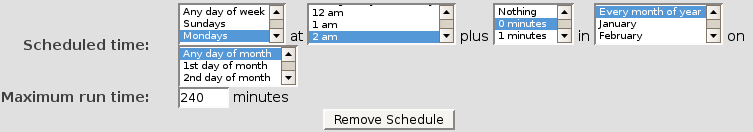
\includegraphics[width=300pt]{sample-schedule}
\end{changemargin}

If you do not have at least one scheduled time, the job will
only run when run manually (see page \pageref{ManageJobs}), and will
not automatically update the index on the appliance based on changes
to the repository.

You can remove a scheduled time by clicking the ``Remove Schedule''
button.

\end{itemize}

\fi

\ifCombinedConnectorGuide
This tab presents scheduling options. Here you can generate one or
more scheduled run times for the job. For a complete description of
the scheduling options, see the description starting on page
\pageref{scheduling}.
\fi

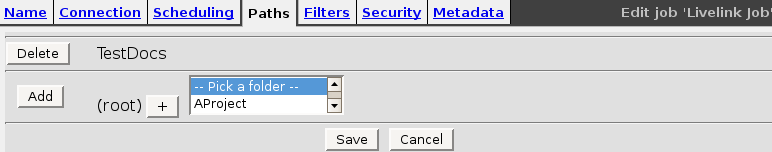
\includegraphics[width=300pt]{edit-job-tab4}

\begin{itemize}

\item \textbf{Roots:} The base directories in Livelink from which you
want your crawl to start. You may select zero, one, or more than one
(though if you select zero, your appliance will not crawl anything). 
To select a directory, select the directory name, click the ``+''
button, and then click ``Add.'' The directory will appear inside the selection
box; you can click the ``Delete'' button next to it to remove it from
your list of directories to be crawled.

\end{itemize}

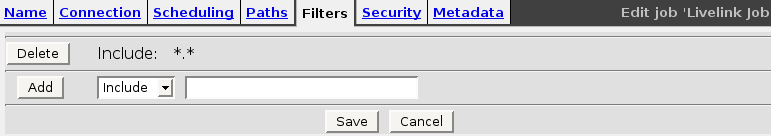
\includegraphics[width=300pt]{edit-job-tab5}

\begin{itemize}

\item \textbf{Filters:} You must define the files that will be 
crawled and indexed during this job. You do this by specifying filetypes
of the form ``\*.XYZ.'' You must specify at least one filetype to 
include, or you will not crawl any documents.

For example, if you want to crawl .QZX
files, you can enter ``\*.QZX'', select ``Include'', and then click Add.
You may define multiple inclusions and exclusions; if an exclusion and an
inclusion conflict, the first one you entered is followed.  

% Licensed to the Apache Software Foundation (ASF) under one or more
% contributor license agreements. See the NOTICE file distributed with
% this work for additional information regarding copyright ownership.
% The ASF licenses this file to You under the Apache License, Version 2.0
% (the ``License''); you may not use this file except in compliance with
% the License. You may obtain a copy of the License at
%
% http://www.apache.org/licenses/LICENSE-2.0
%
% Unless required by applicable law or agreed to in writing, software
% distributed under the License is distributed on an ``AS IS'' BASIS,
% WITHOUT WARRANTIES OR CONDITIONS OF ANY KIND, either express or implied.
% See the License for the specific language governing permissions and
% limitations under the License.

MetaCarta GTS currently supports the following filetypes:

\begin{itemize}
\item ASCII Text Files with or without extensions (.txt, etc...)
\item HTML Documents (.htm, .html)
\item Adobe\circler\ Acrobat\circler\ files (.pdf)
\item Adobe PostScript\circler\ files (.ps)
\item Microsoft\circler\ Word\circler\ documents (.doc)
\item Microsoft Excel\circler\ spreadsheets (.xls)
\item Microsoft PowerPoint\circler\ presentations (.ppt)
\item Rich Text Format documents (.rtf)
\end{itemize}

\note{Documents larger than 50MB are converted to plaintext and then truncated to 50MB.} 



To crawl and index all files, enter ``\*.\*'' and click Add.

\end{itemize}

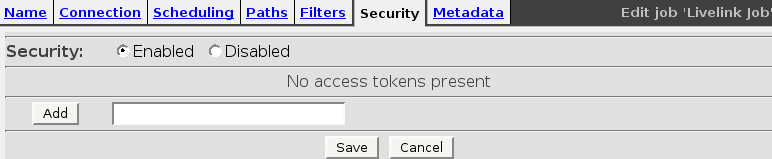
\includegraphics[width=300pt]{edit-job-tab6}

\begin{itemize}

\item \textbf{Security:} Allows you to control whether or not file ACLs,
or access control lists, are passed to the appliance with the files. If
you select ``Disabled'' here, all files crawled from Livelink will be
visible to all GTS users.

\item \ifLivelinkGuide \label{ForceACL}\fi \textbf{Access Tokens:} If you want to pass on
your own Active Directory ACLs instead of those used by Livelink---or
your Livelink instance does not contain Livelink ACLs---you can enter
them here.  You should enter one or more SIDs that you want to have
read permissions on the files crawled in this job. Two special
Livelink tokens can also be entered. The token ``SYSTEM'' represents
Livelink system administrators, while the token ``GUEST'' represents
users logged into Livelink as guests. For more information about AD
ACLs and SIDs, please see the security sections of the
\documentref{MetaCarta Appliance Administrator's Guide}.

\note{If you have disabled security, these ACLs will not be passed to
the appliance.}

\end{itemize}

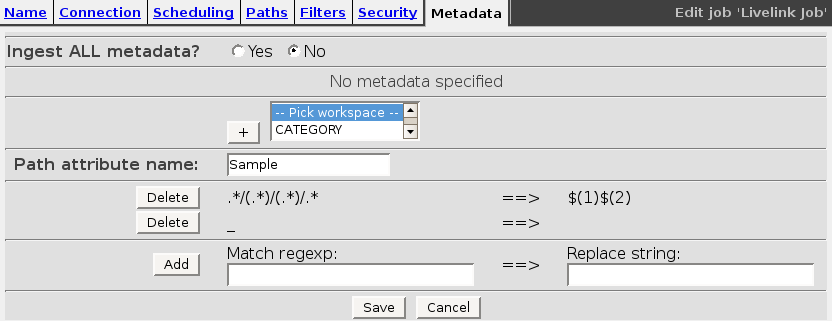
\includegraphics[width=300pt]{edit-job-tab7}

\begin{itemize}

\item \textbf{Ingest ALL metadata:} Choose yes if you want to ingest all 
metadata for each document crawled.

\item \textbf{Metadata:} The Livelink server stores various metadata
information about documents in its index.  You can select those metadata
fields here and have them sent along with the files you index as metadata.
Metadata will not be geographically parsed or used to create the index
on the MetaCarta appliance; however, with the SOAP Search API, you
can construct searches based specifically on this metadata. For more
information on the SOAP Search API, please see the \documentref{MetaCarta
SOAP Search API Guide}.

\item \textbf{Path attribute name:} The name of the GTS metadata
attribute to which you want to attach Livelink file path data, if any.

\item \textbf{Path-value mapping:} The regular expressions
and substitutions that you want to use to collect information
from the Livelink file path. Using the regular expression
rules on page \pageref{regex}, you can construct one or more
expressions. In the example shown, there are two expressions. The
first, \verb+.*/(.*)/(.*)/.*+ to \verb+$(1) $(2)+, would change the
directory path ``Project/Folder\_1/Folder\_2/ Filename'' into ``Folder\_1
Folder\_2.'' The second, \_ to a space, would then be applied to turn
the metadata into ``Folder 1 Folder 2.'' It is important to allow more
than one transform so that you can, if necessary, extract text data and
then parse the extracted data. The end result of the last transform will
be ingested as the value of the metadata attribute defined previously.

\end{itemize}

After entering this information, you will be taken to the status page
for this job:

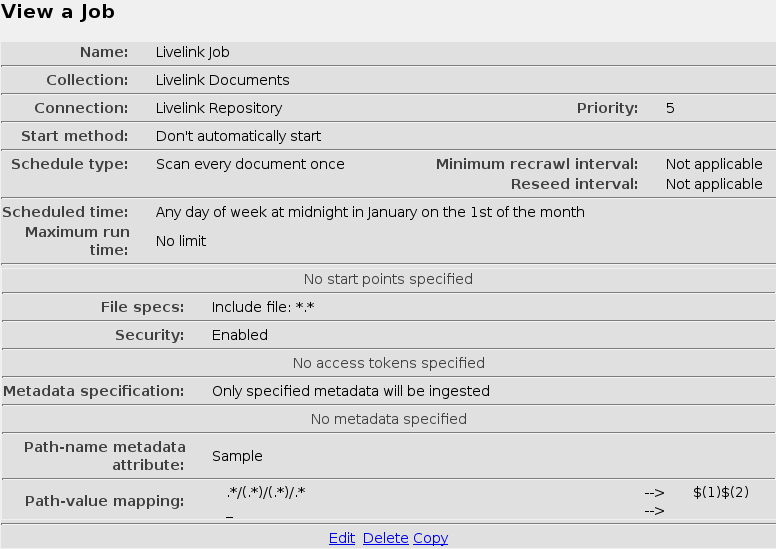
\includegraphics[width=300pt]{view-job-status}
